\documentclass{article}
\usepackage{graphicx} % Required for inserting images
\usepackage[spanish]{babel}
\usepackage{listings}
\usepackage{xcolor}
\usepackage{courier}

\lstdefinestyle{mystyle}{
    backgroundcolor=\color{gray!10},   % Color de fondo
    commentstyle=\color{green!60!black}, % Color de comentarios
    keywordstyle=\color{blue},         % Color de palabras clave
    numberstyle=\tiny\color{gray},     % Estilo de números de línea
    stringstyle=\color{red},           % Color de strings
    basicstyle=\ttfamily\footnotesize, % Fuente del código
    breakatwhitespace=false,           
    breaklines=true,                   % Permite salto de línea automático
    captionpos=b,                      % Posición del caption
    keepspaces=true,                   
    numbers=left,                      % Números de línea a la izquierda
    numbersep=5pt,                     
    showspaces=false,                  
    showstringspaces=false,
    showtabs=false,                    
    tabsize=2,
    frame=single,                      % Marco alrededor del código
    rulecolor=\color{black!30}         % Color del marco
}

\lstset{style=mystyle}

\title{Práctica 2: Sockets}
\author{Laura Itzel Rodríguez Dimayuga}
\date{\today}
 
\begin{document}

\maketitle

\section{Introducción}

\begin{enumerate}
    \item Instalar Sudo
    \begin{figure}
        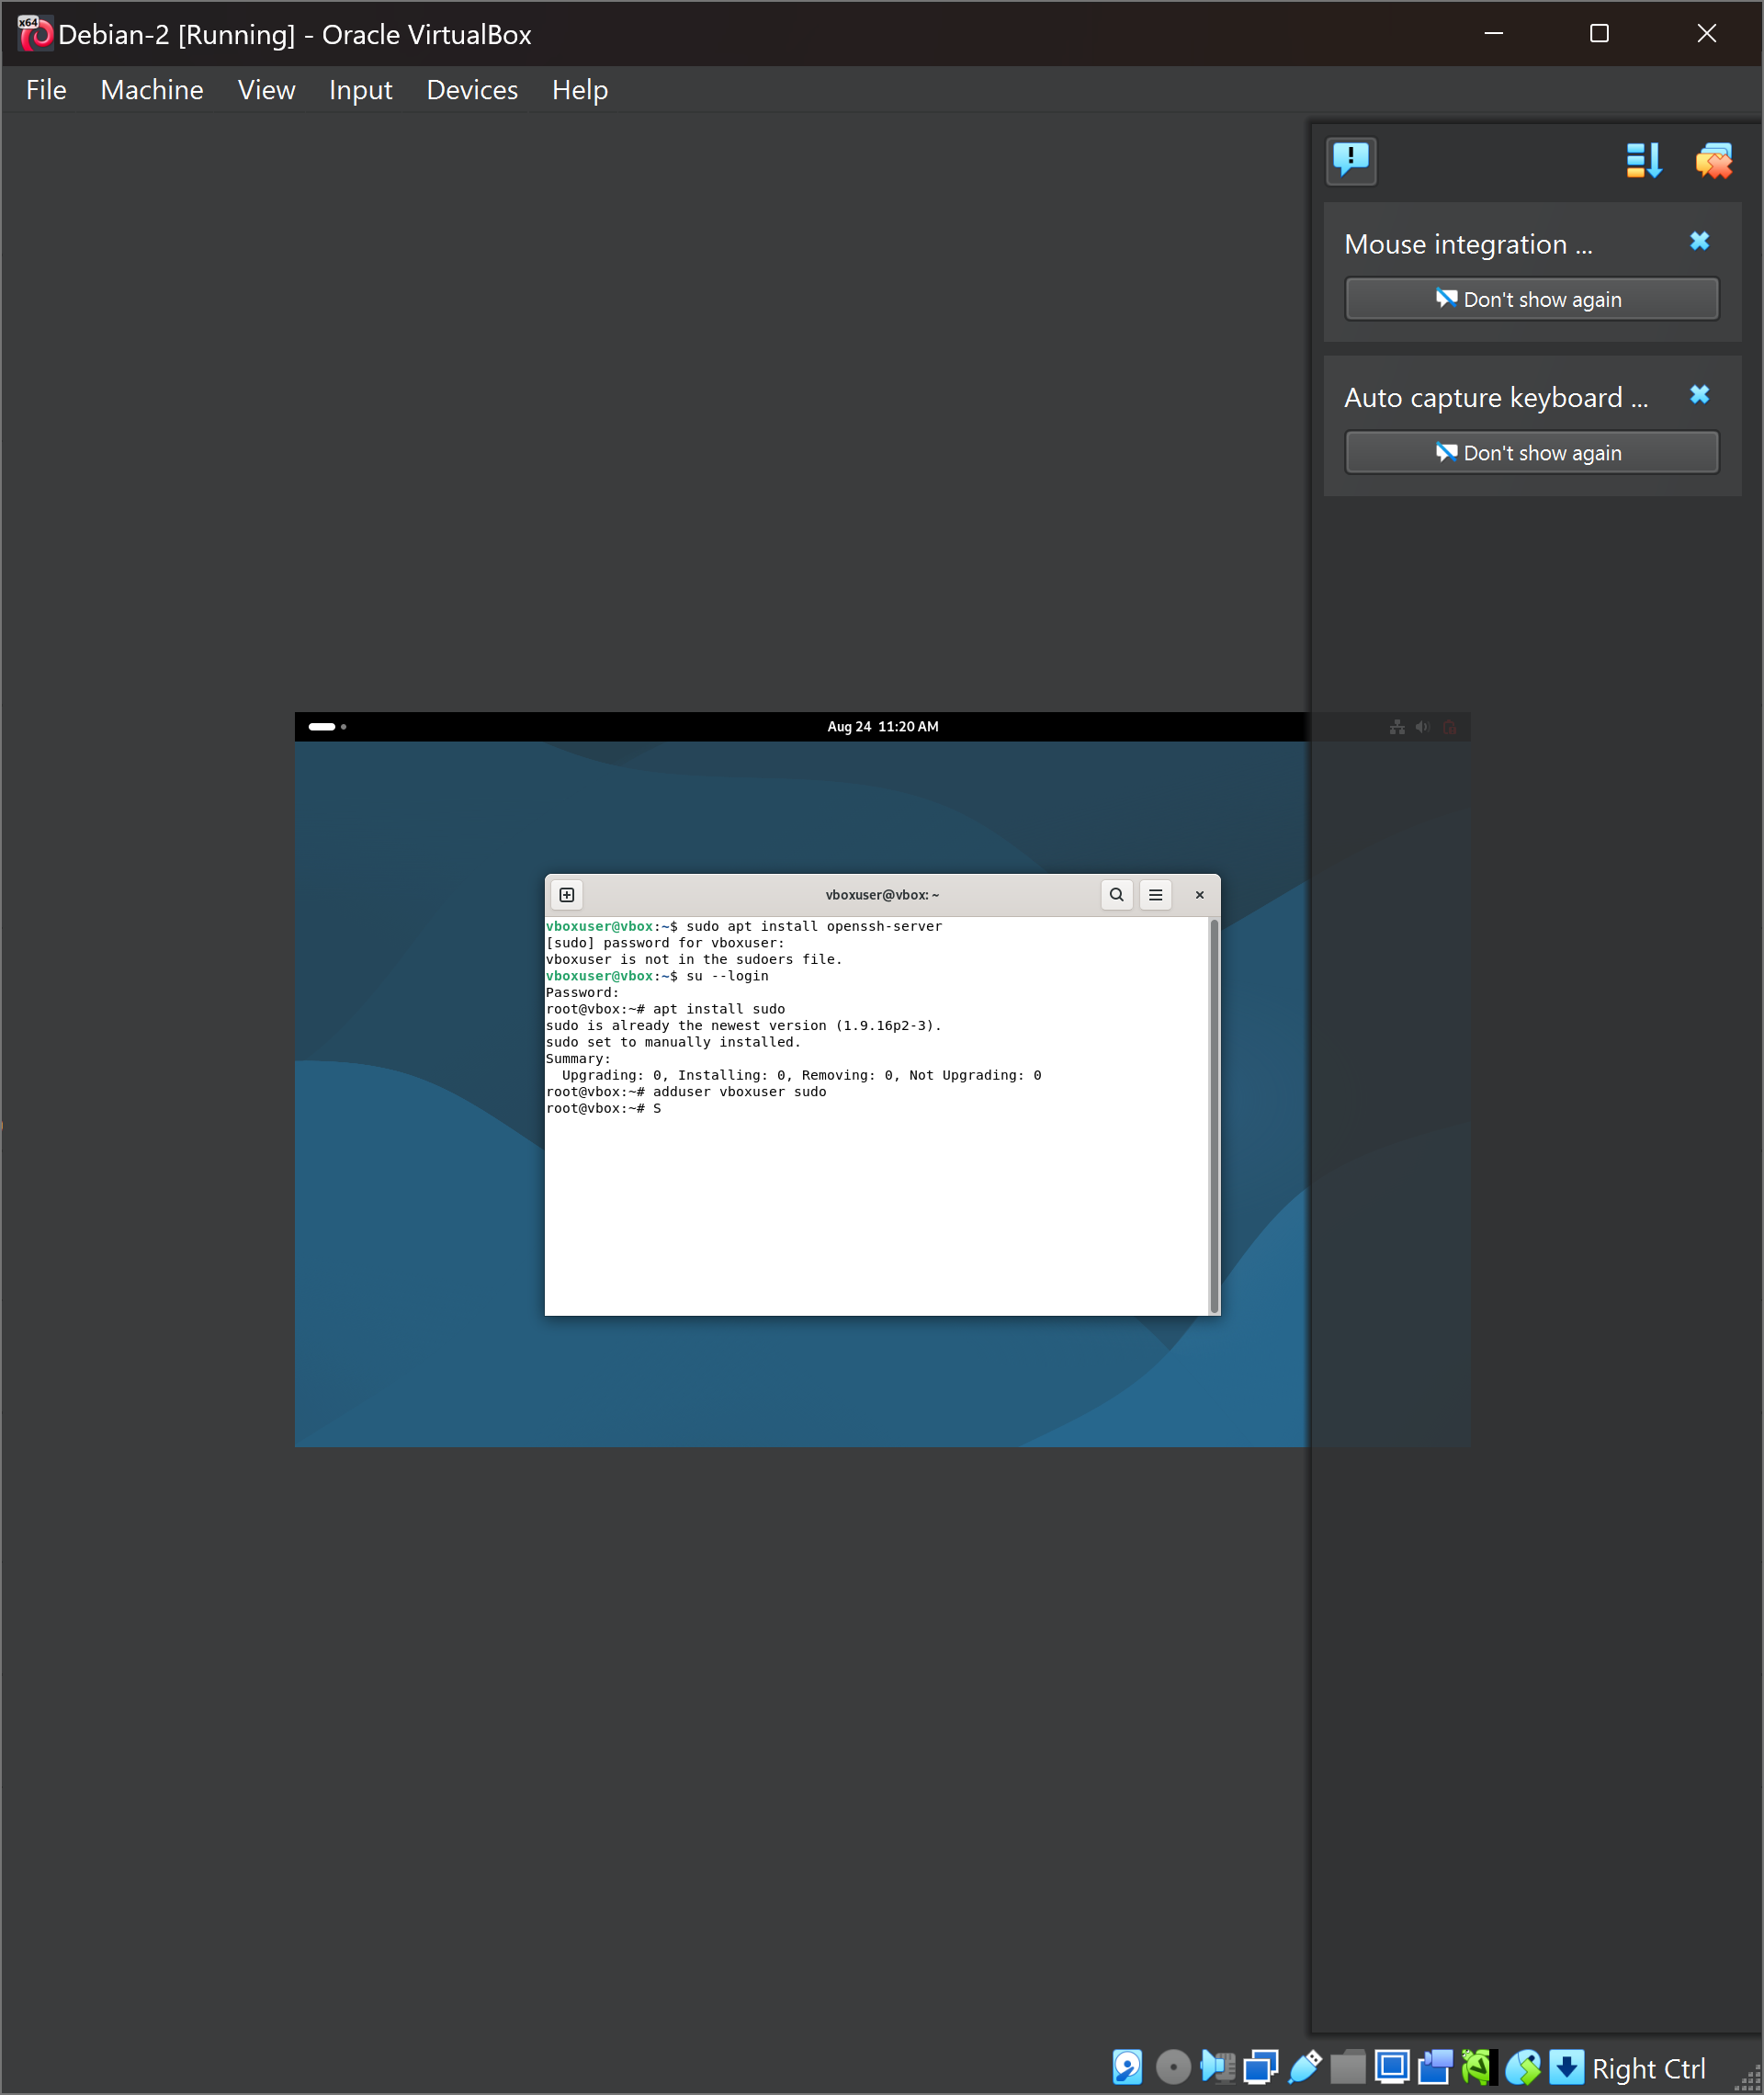
\includegraphics[width=\linewidth]{./images/install_sudo.png}
        \caption{Instalación de Sudo}
    \end{figure}
    \begin{lstlisting}[language=bash]
    # nos cambiamos al root 
    $ su --login 
    Password: 
    # instalamos sudo 
    $ apt install sudo 
    # anadimos el usuario laudima al grupo sudo
    $ adduser laudima sudo
    \end{lstlisting}
    \item  Ahora en ambas maquinas instale el paquete openssh-server y verificamos la ip
    \begin{lstlisting}[language=bash]
    $ apt install openssh-server
    $ ip a
    \end{lstlisting}
    \begin{figure}
        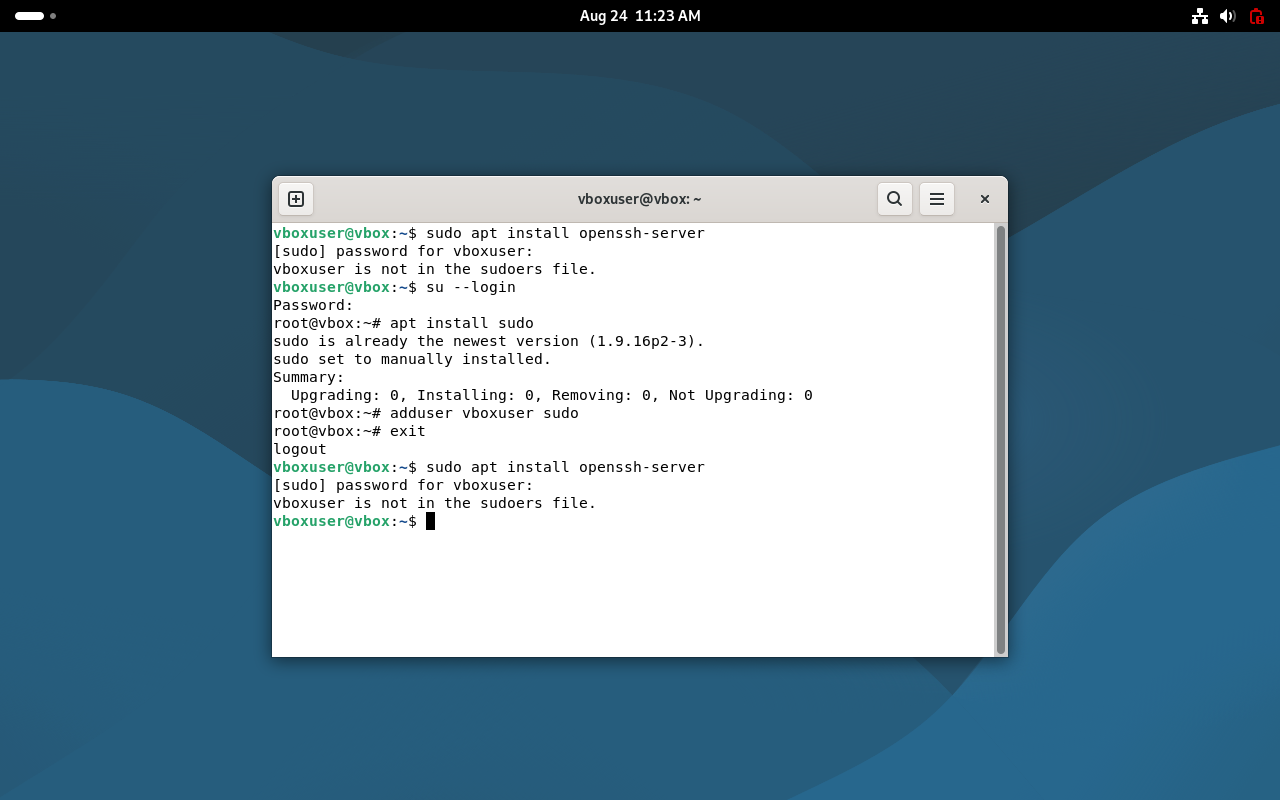
\includegraphics[width=\linewidth]{./images/install-open-ssh.png}
        \caption{Instalación de OpenSSH}
    \end{figure}
    \begin{figure}
        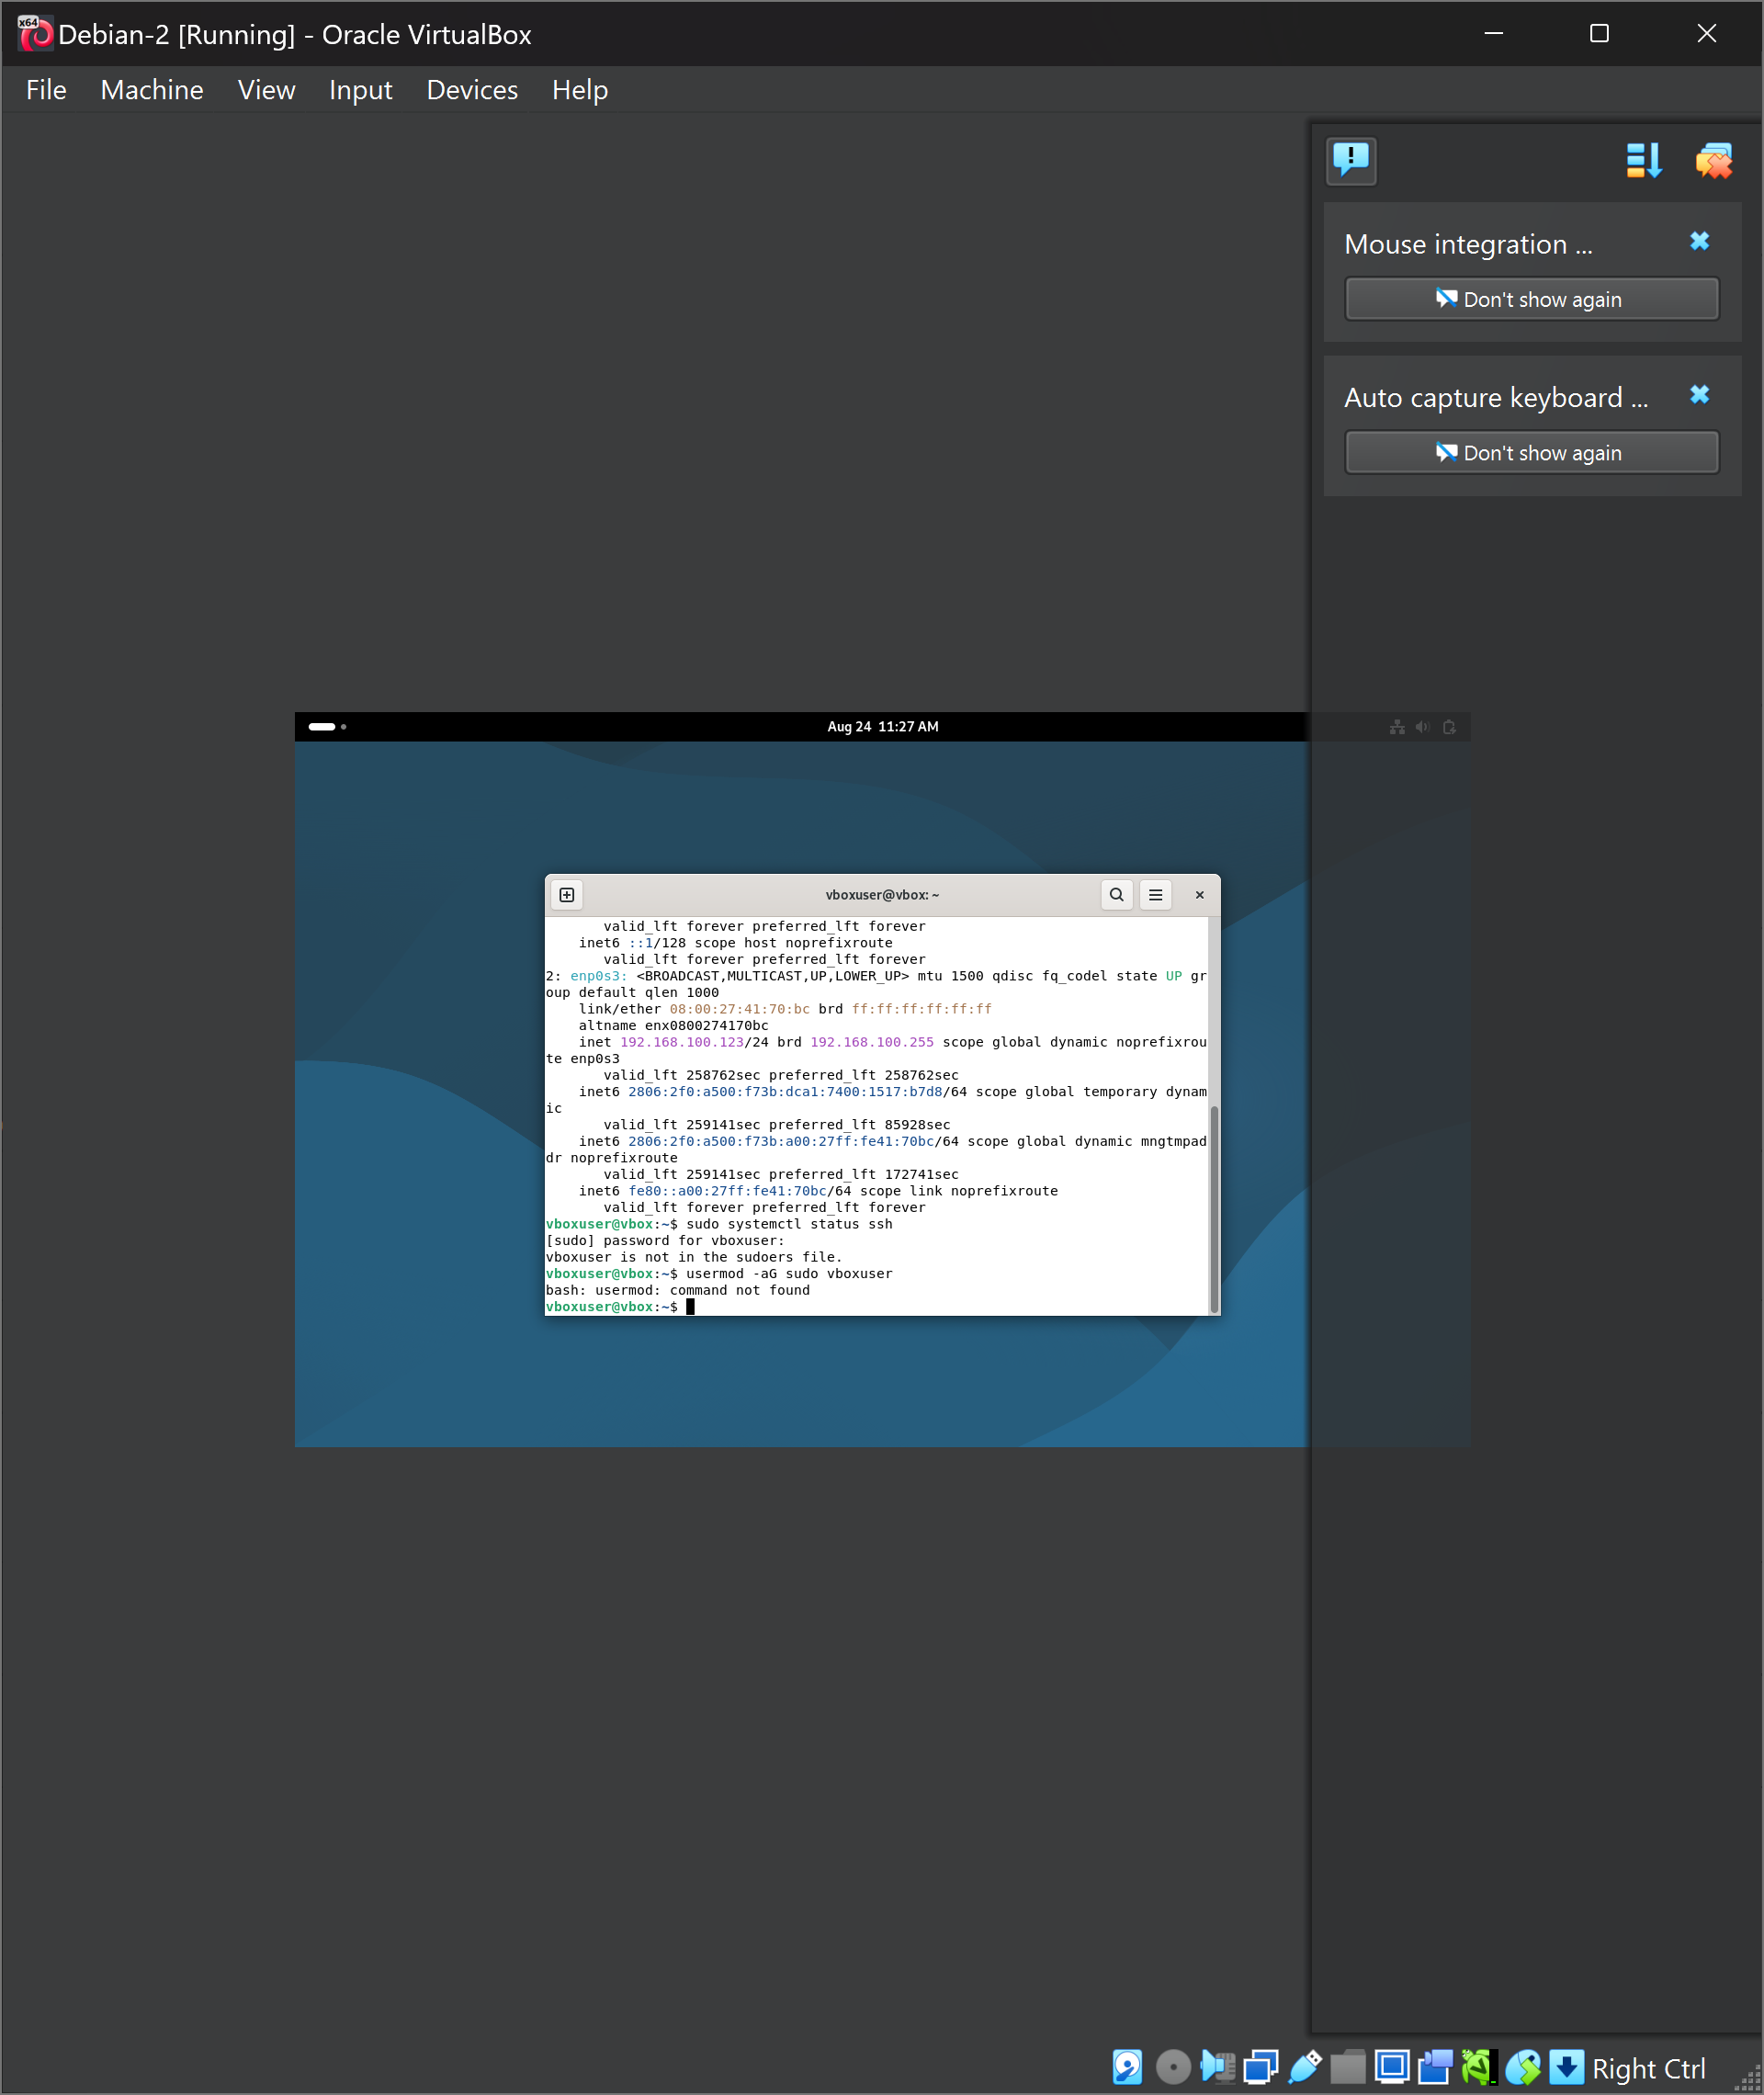
\includegraphics[width=\linewidth]{./images/ipa.png}
        \caption{Verificación de IP}
    \end{figure}
    \item En ambas máquinas habilite el ssh. Y cheque su estatus.
    \begin{lstlisting}[language=bash]
    $ sudo systemctl enable ssh
    $ sudo systemctl start ssh
    $ sudo sys
    temctl status ssh
    \end{lstlisting}
    \begin{figure}
        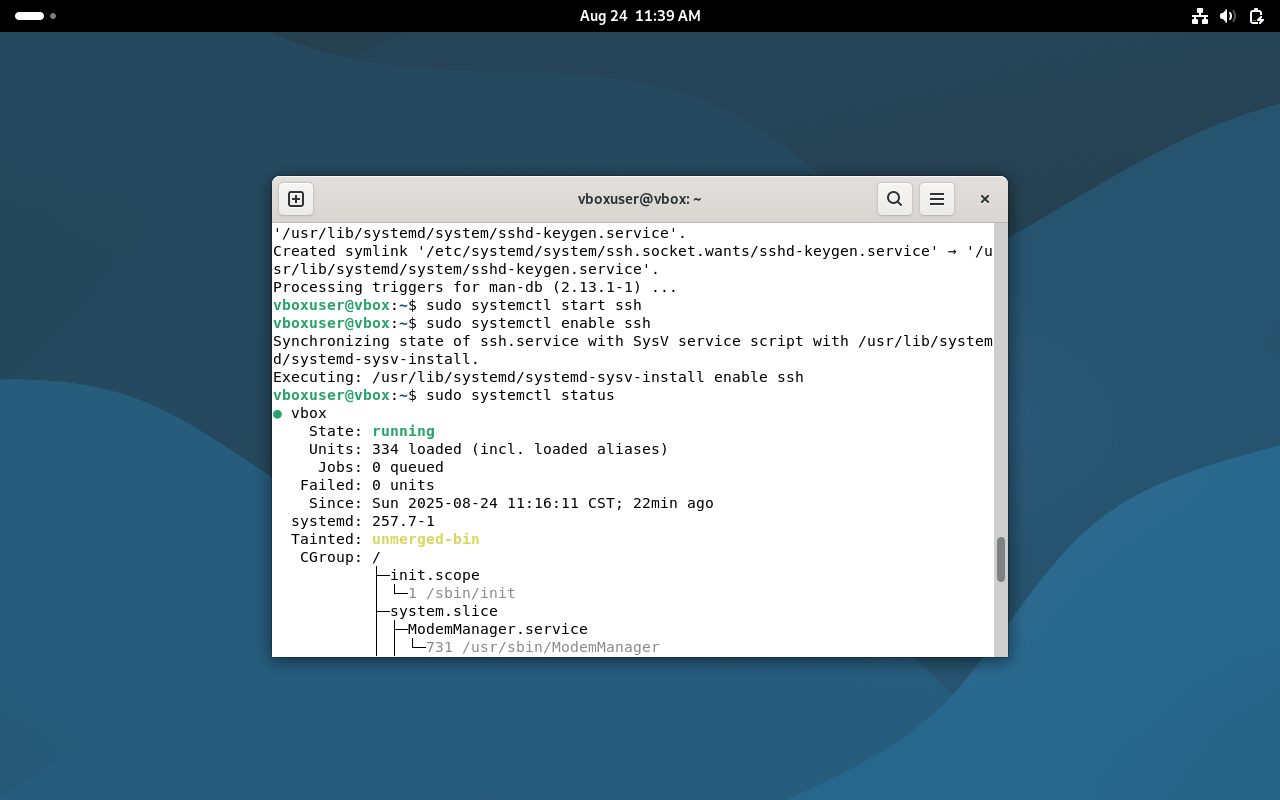
\includegraphics[width=\linewidth]{./images/ssh-status.png}
        \caption{Estado del servicio SSH en Debian}
    \end{figure}
    \begin{figure}
        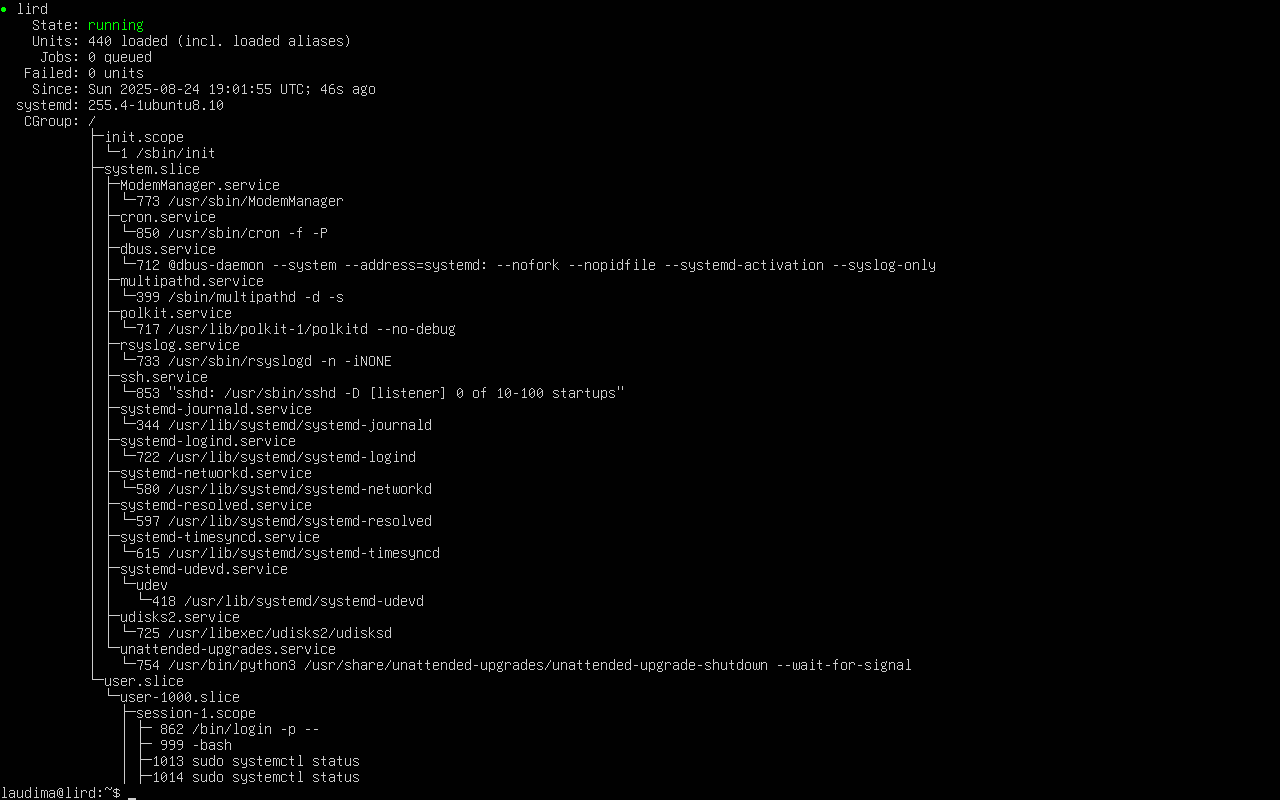
\includegraphics[width=\linewidth]{./images/ssh-status-ubuntu.png}
        \caption{Estado del servicio SSH en Ubuntu}
    \end{figure}
    \item Em ambas maquinas installe los paquetes para poder correr C, con 
    \begin{lstlisting}[language=bash]
    $ sudo apt install build-essential
    $ gcc --version
    \end{lstlisting}
    \item En mi máquina de ubuntu escribí el archivo \texttt{server.c} y descargué el archivo \texttt{cipherworlds.txt} desde el repositorio.
    \item En mi máquina de debian escribí el archivo \texttt{client.c}. 
    \item En ambas máquinas compilé los archivos con el siguiente comando:
    \begin{lstlisting}[language=bash]
    $ gcc -o server server.c
    $ gcc -o client client.c
    \end{lstlisting}
    \item Verifique que el puerto 7006 esté abierto.
    \begin{figure}
        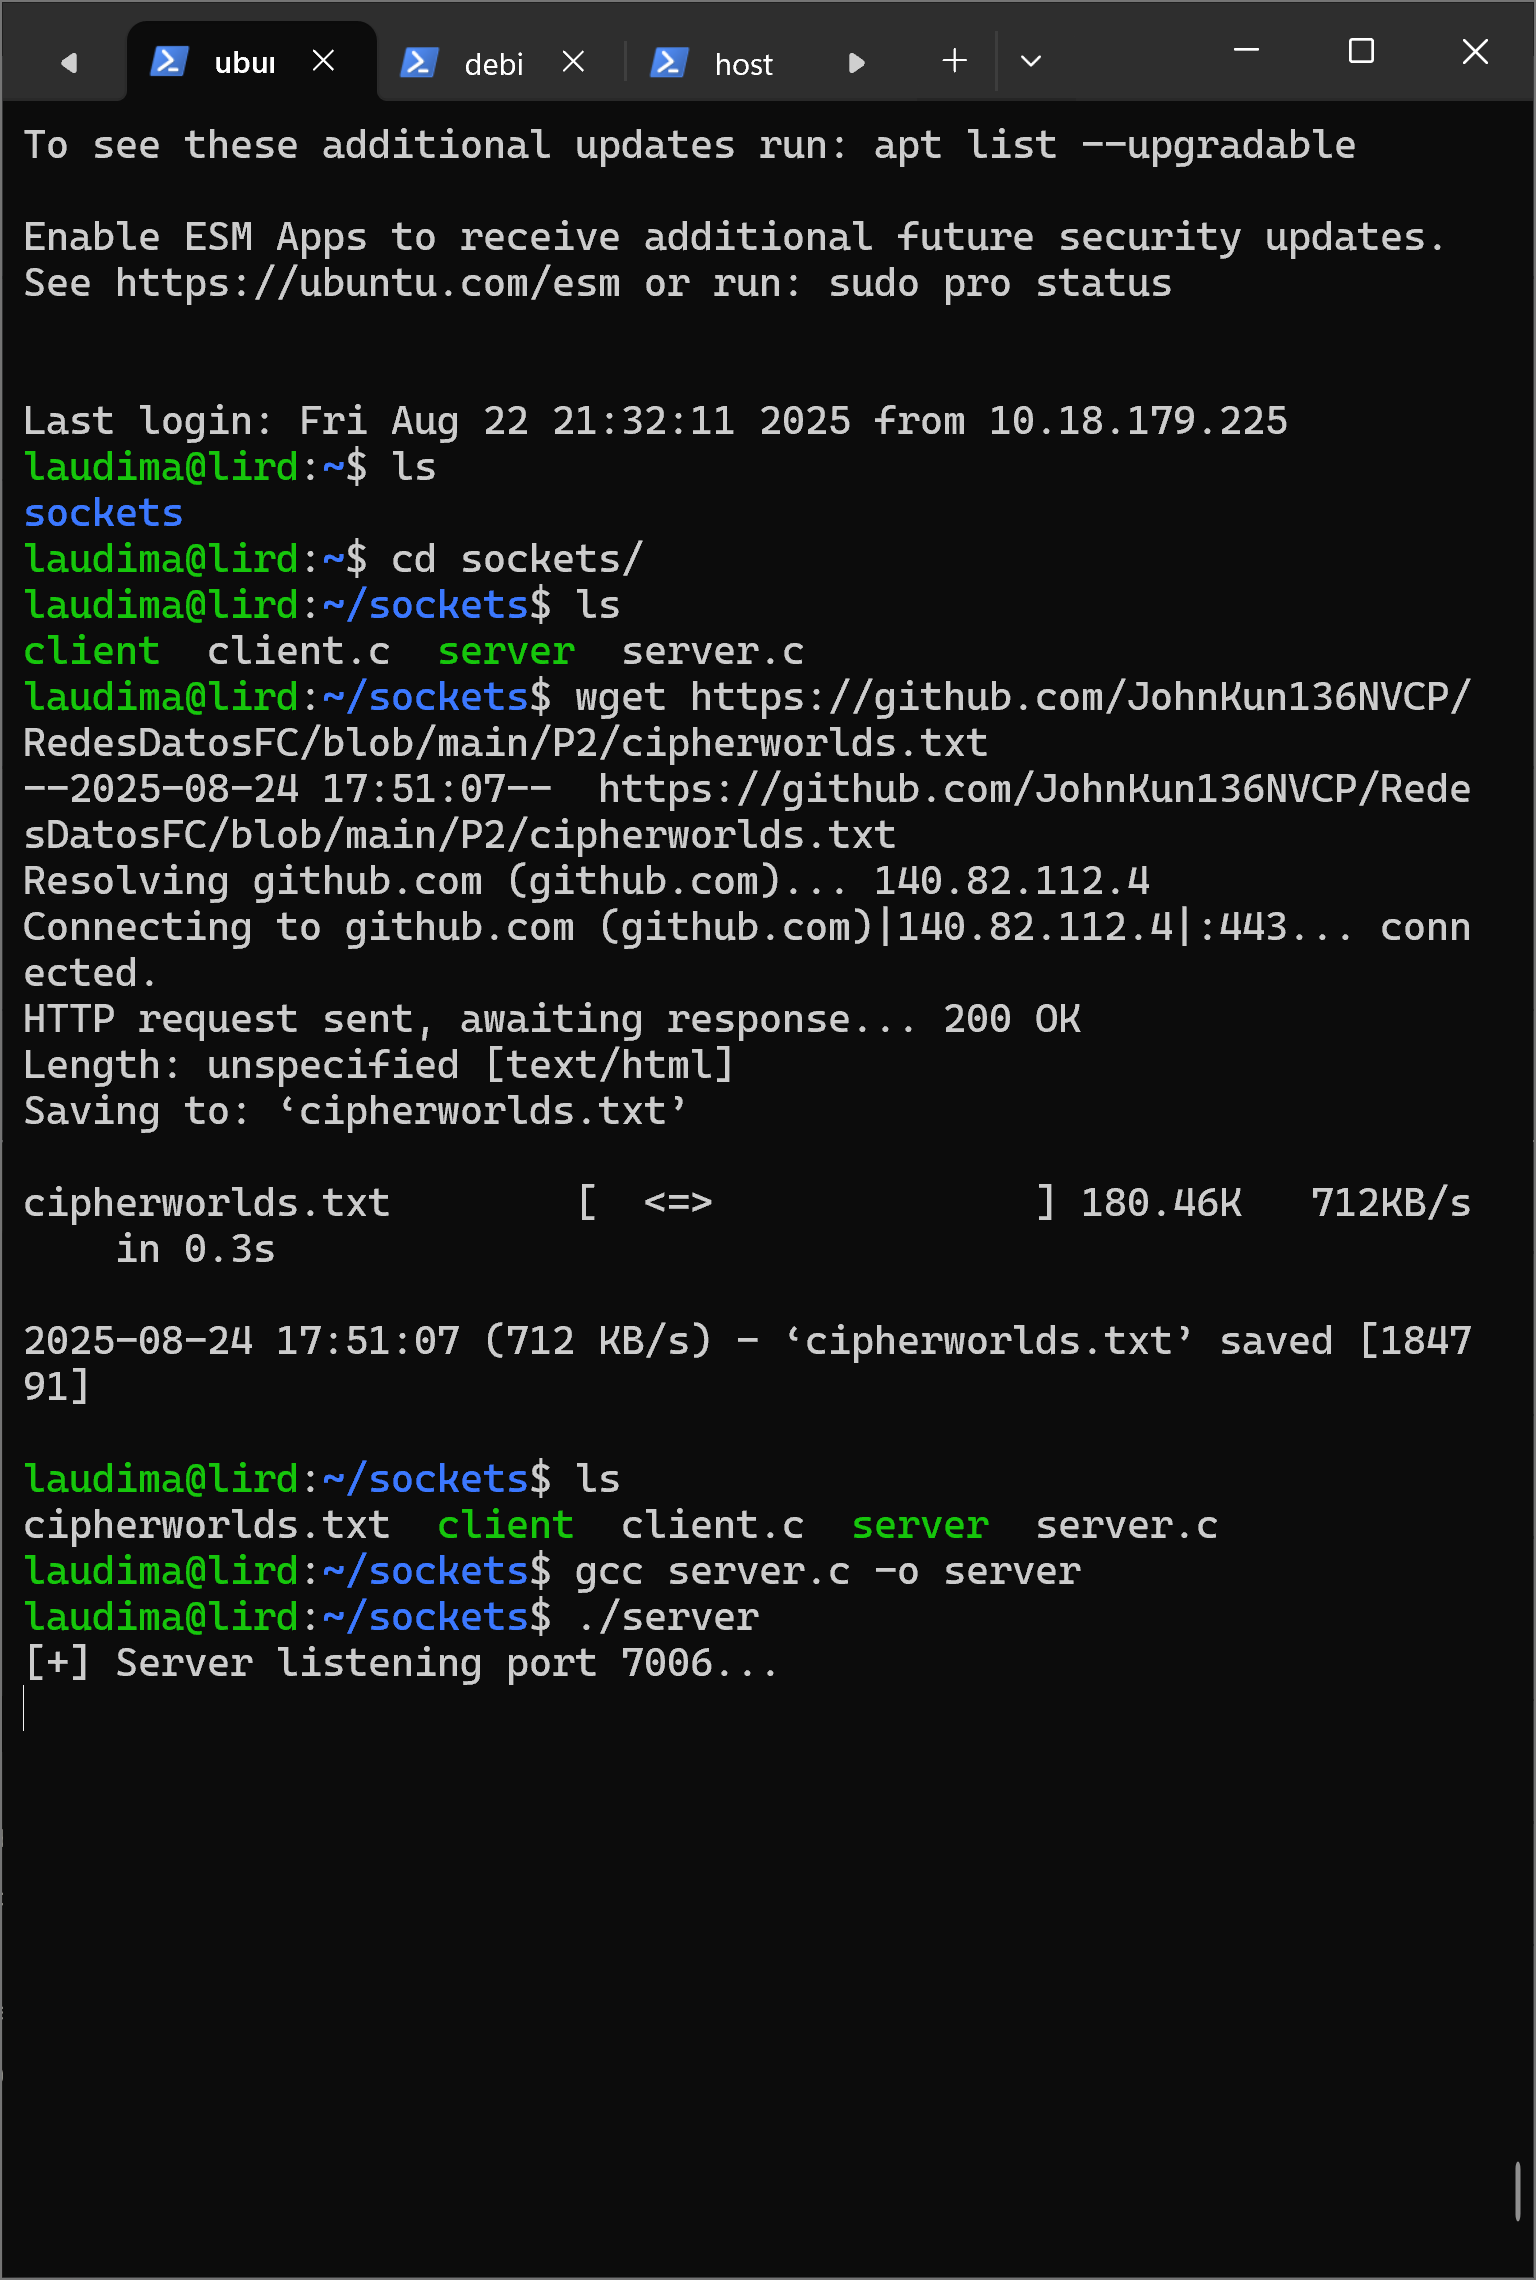
\includegraphics[width=\linewidth]{./images/puerto1.png}
        \caption{Verificación de puerto en Ubuntu}
    \end{figure}
    \begin{figure}
        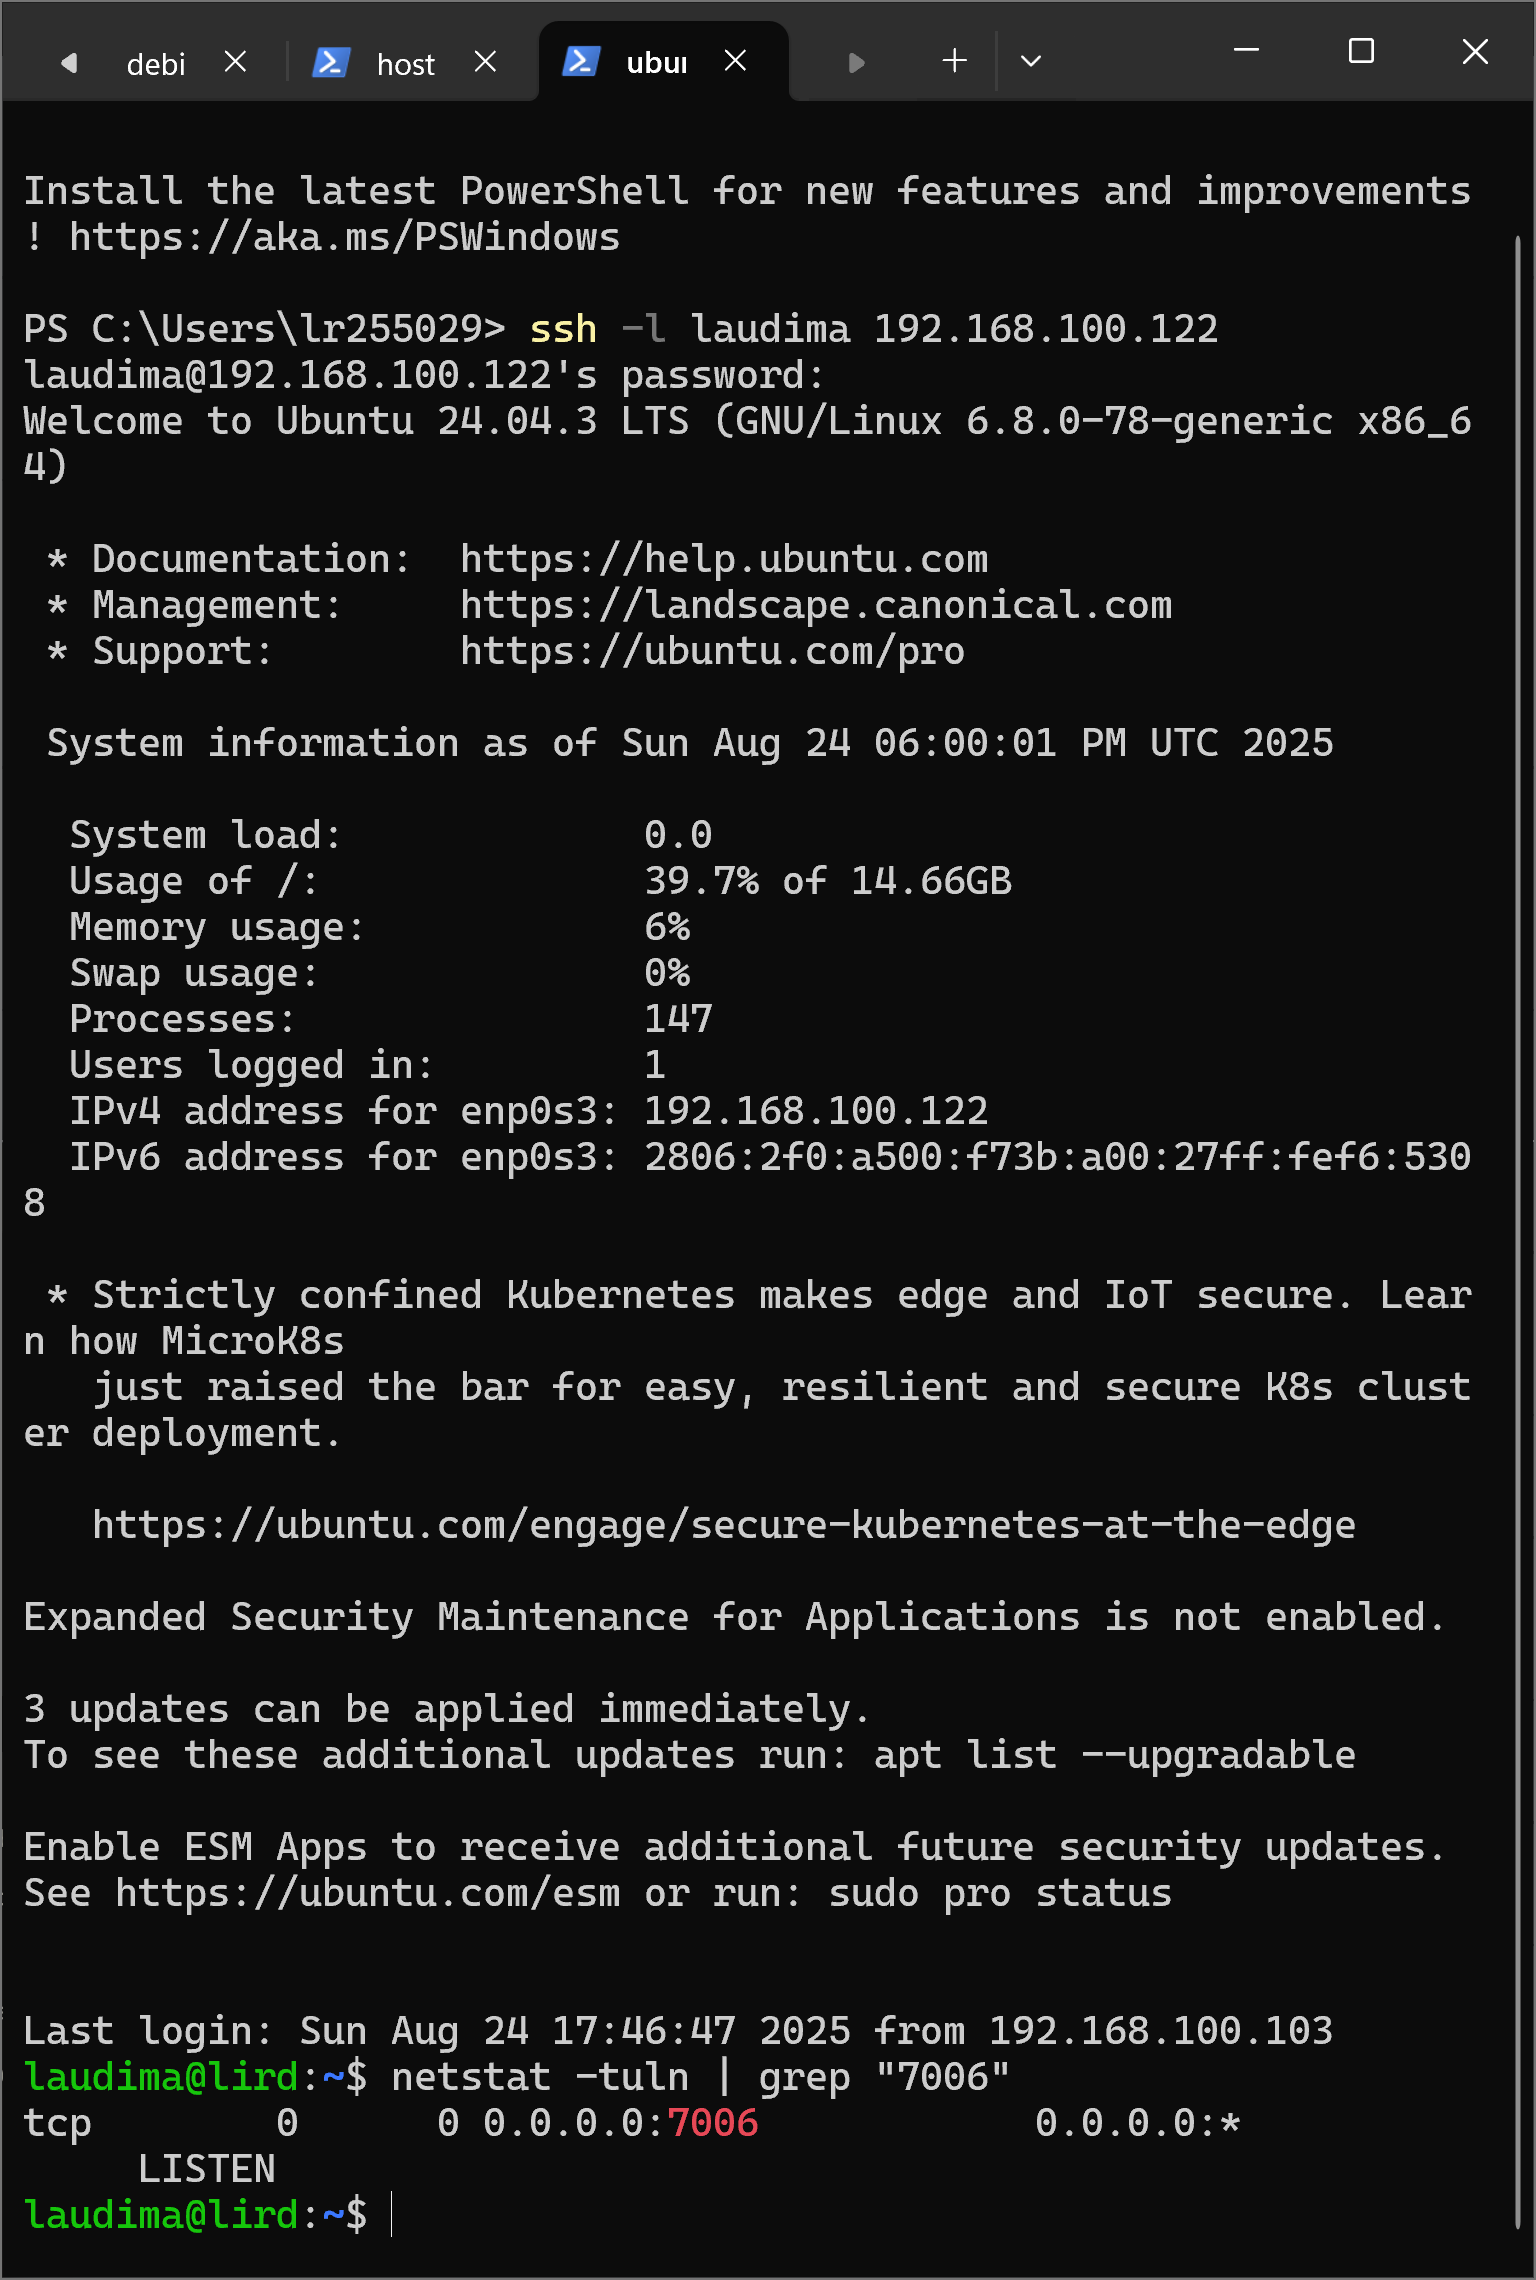
\includegraphics[width=\linewidth]{./images/puerto.png}
        \caption{Verificación de puerto en  ubuntu pero desde otra terminal}
    \end{figure}
    \item En la máquina de debian corrí el siguiente comando:
    \begin{lstlisting}[language=bash]
    $ ./client <key> <shift> 
    \end{lstlisting}

    Y pude lograr decifrar el mensaje
    \begin{figure}
        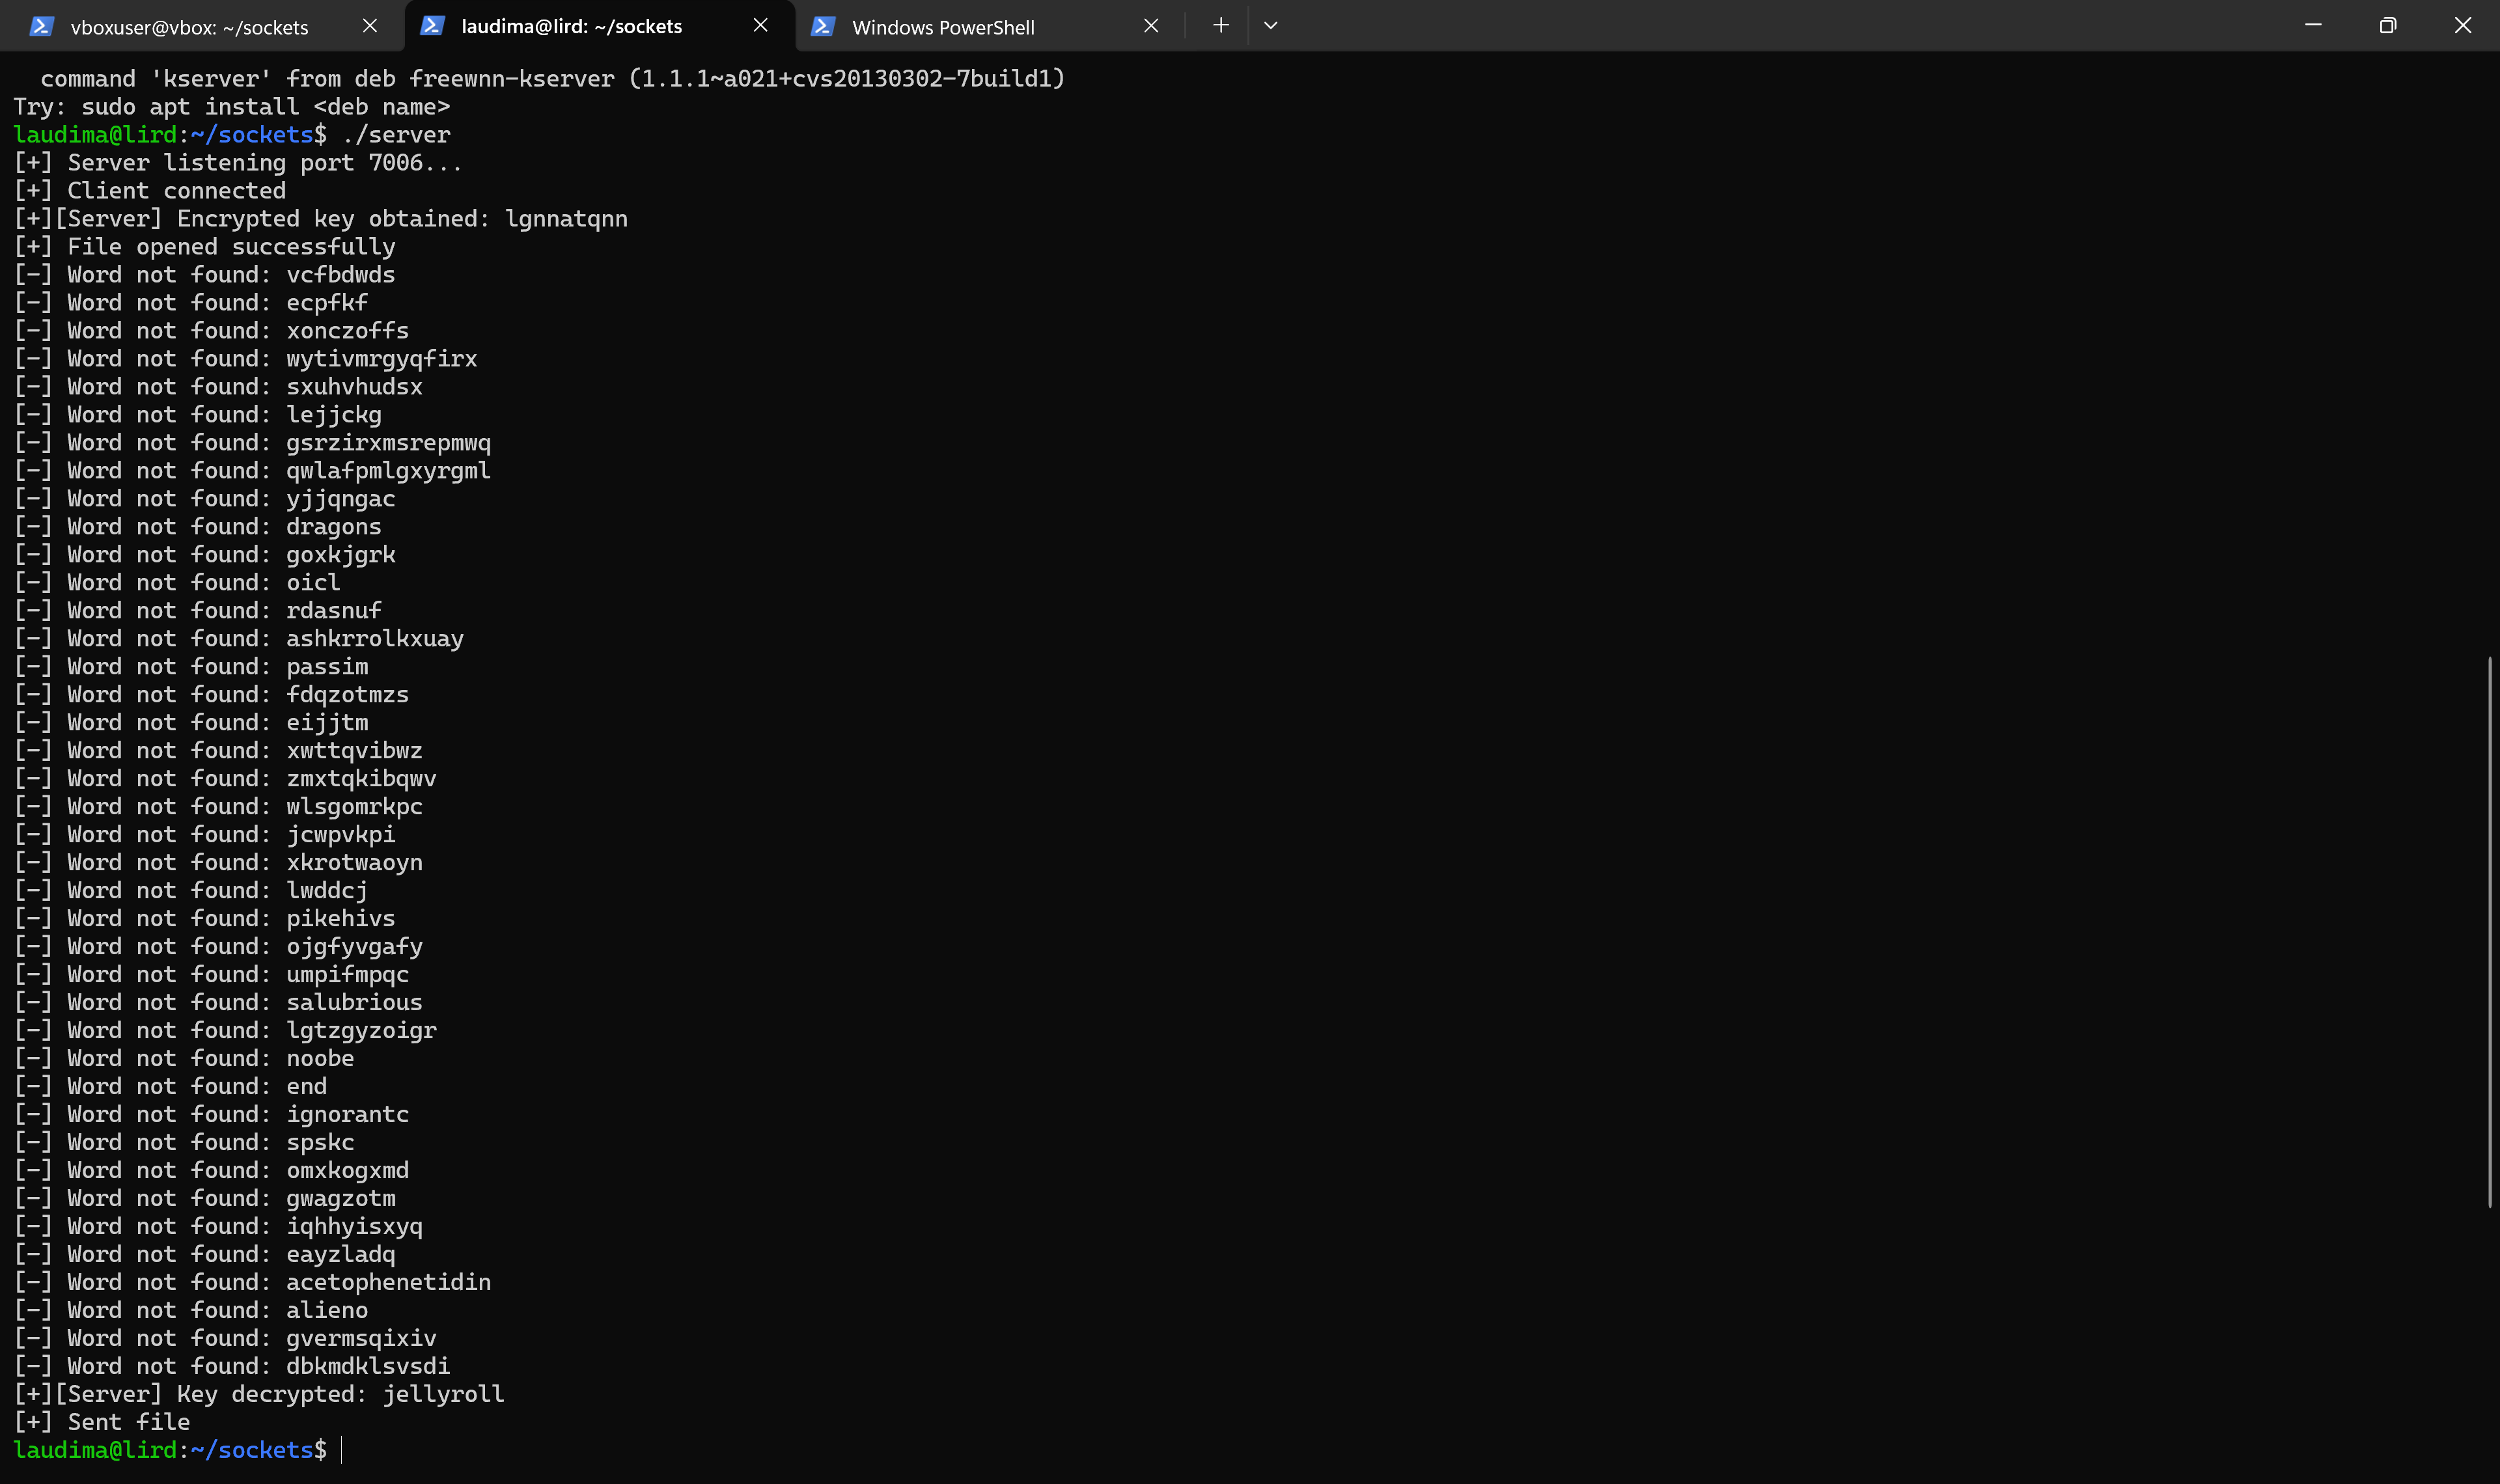
\includegraphics[width=\linewidth]{./images/server.png}
        \caption{Servidor en ejecución}
    \end{figure}
    \begin{figure}
        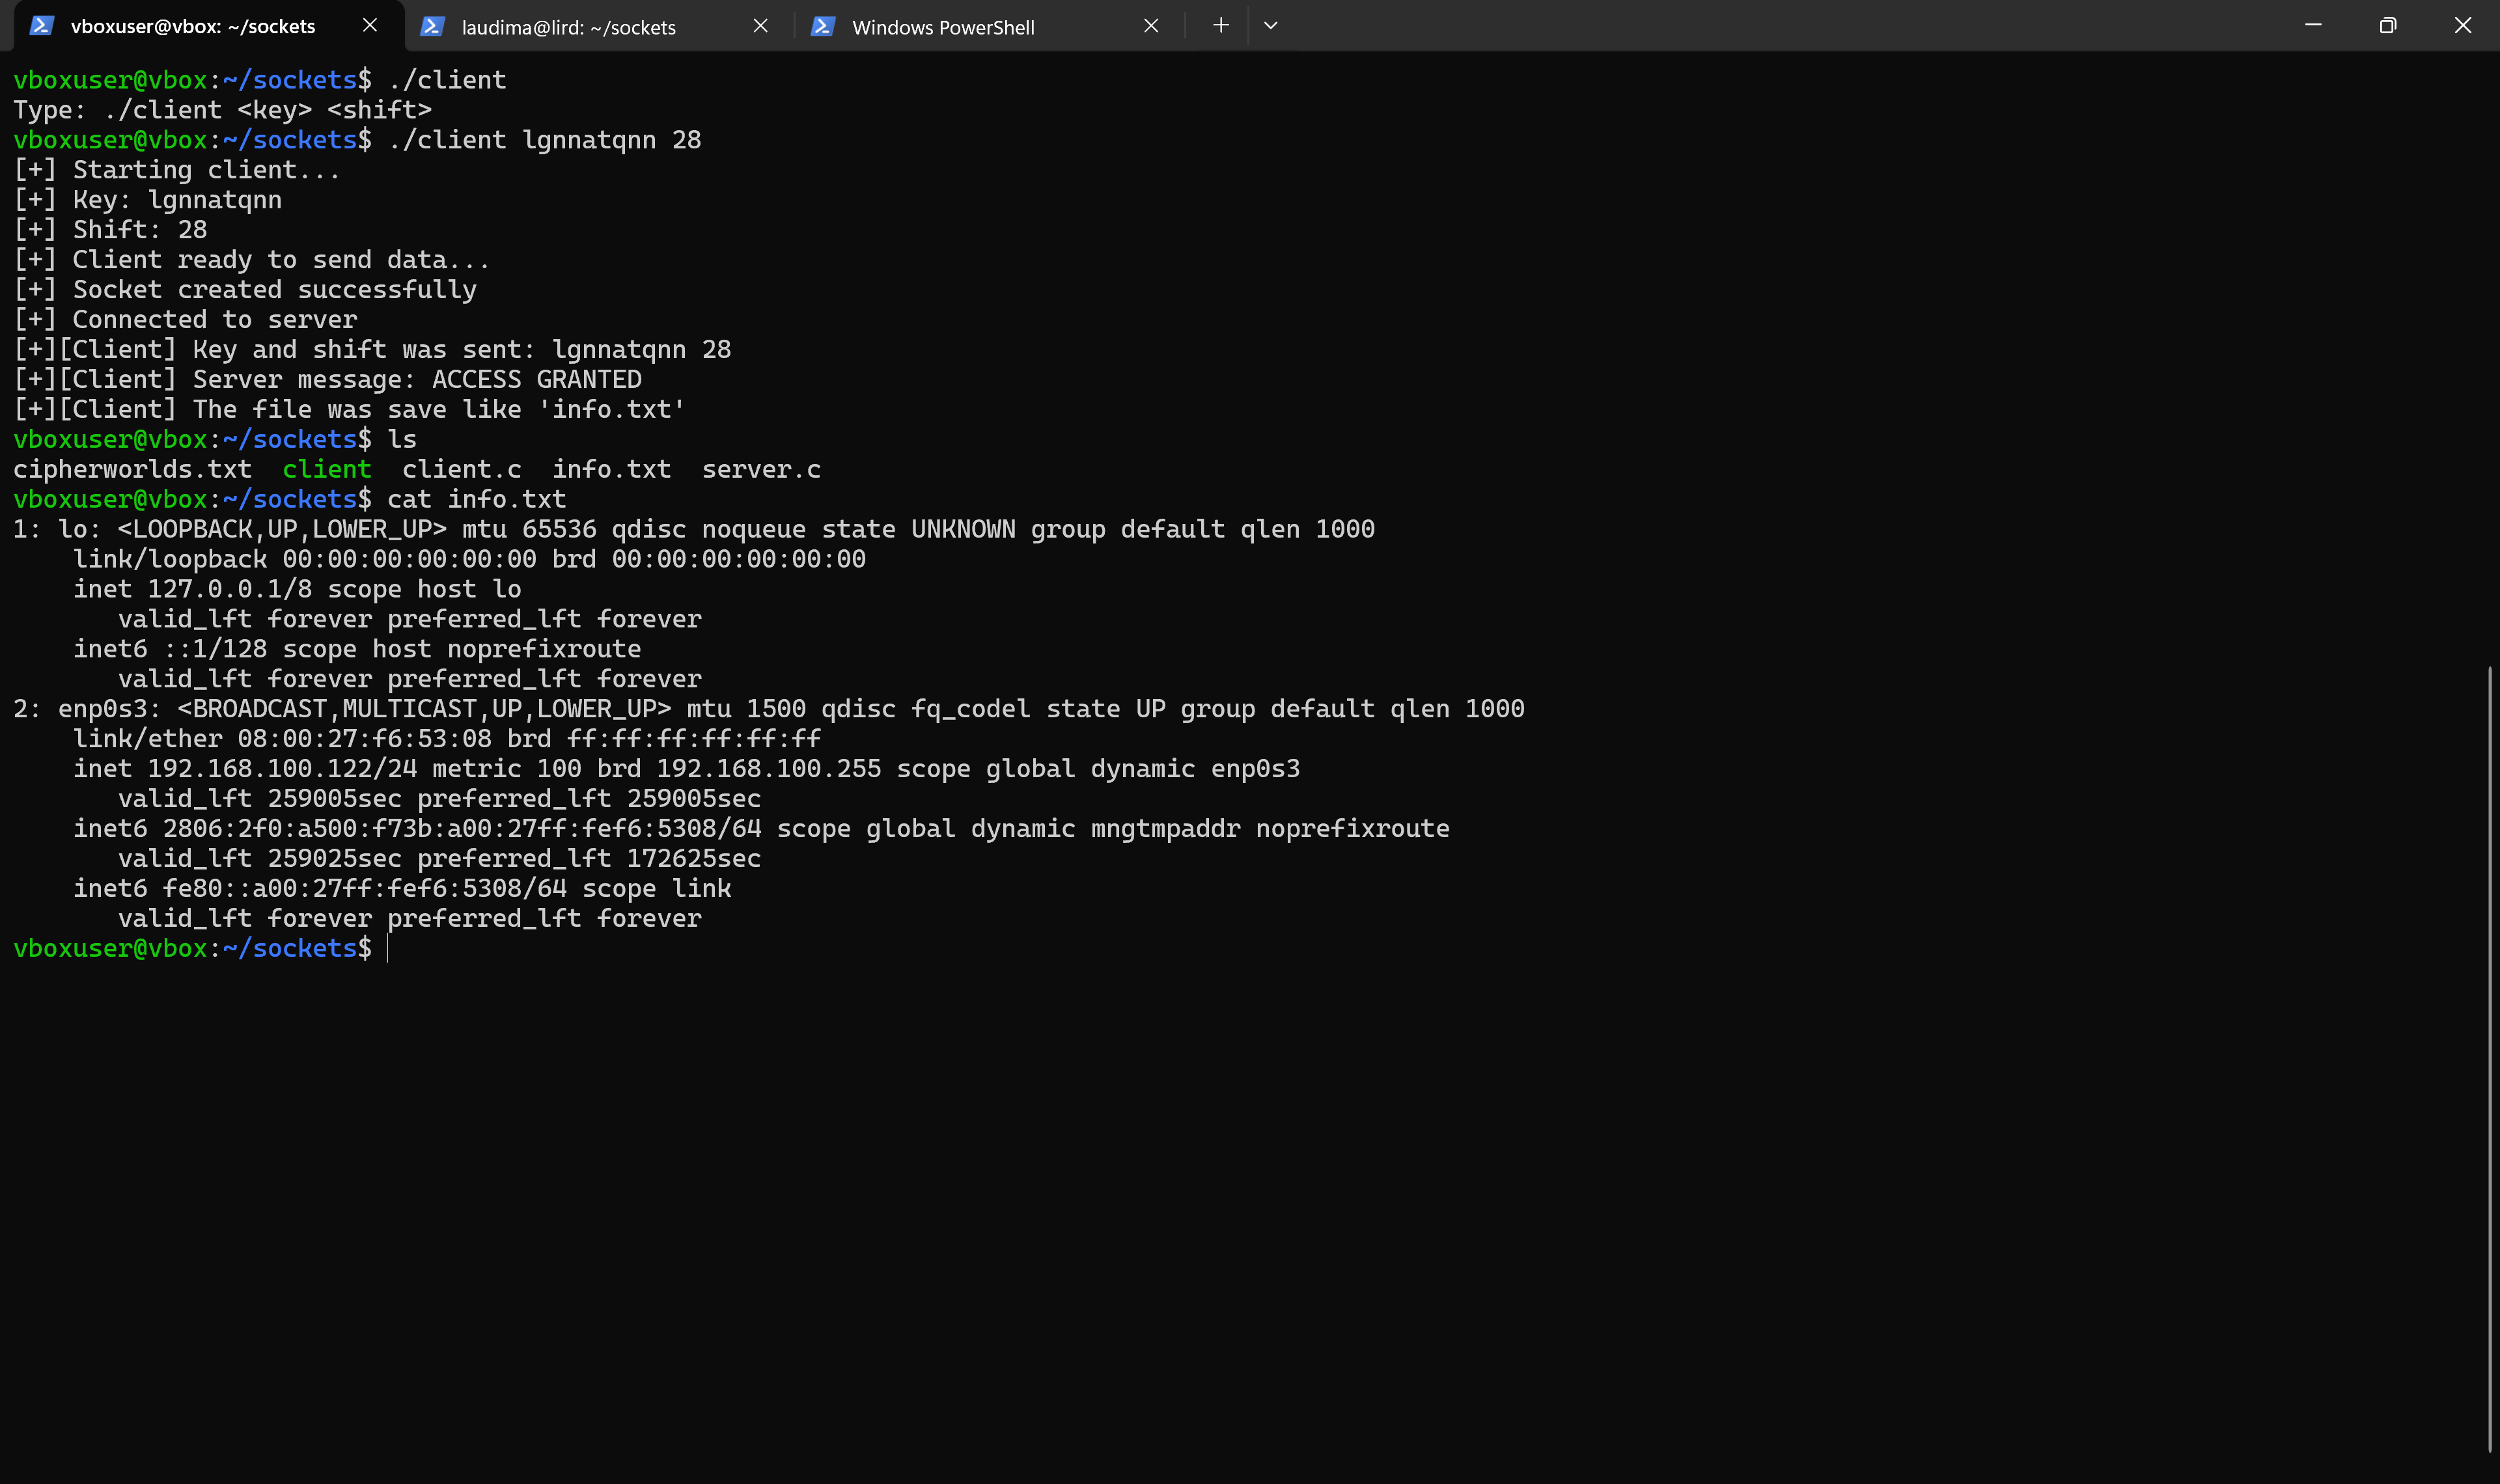
\includegraphics[width=\linewidth]{./images/client.png}
        \caption{Cliente en ejecución}
    \end{figure}
\end{enumerate}
\section{Teoría}
\begin{enumerate}
    \item ¿Para qué sirven las bibliotecas arpa-inet.h, sys-socket.h, netinet-in.h, unistd.h, ctype.h?
    \begin{itemize}
        \item \texttt{arpa-inet.h}: definiciones para operaciones de Internet
        \item \texttt{sys-socket.h}: Contiene definiciones 
        relacionadas con la creación y manejo de sockets.
        \item \texttt{netinet-in.h}: Define las estructuras de datos y 
        funciones específicas para el manejo de direcciones IP y protocolos de red.
        \item \texttt{unistd.h}: Proporciona acceso a las llamadas al 
        sistema POSIX, incluyendo funciones para manejar archivos y procesos.
        \item \texttt{ctype.h}: Contiene funciones para la manipulación de 
        caracteres, como la verificación de tipos de caracteres (por ejemplo, si es 
        un dígito o una letra).
    \end{itemize}
    \item ¿Qué tipo de Socket se creó en esta práctica? ¿UDP, TCP? Si es alguno de esos dos o los dos
explica por qué.

Como ocupamos \texttt{SOCK STREAM} se creó un socket TCP, ya que este tipo de socket proporciona una conexión orientada a la conexión y garantiza la entrega de datos en el orden correcto.

\item ¿Qué hacen fgets y sizeof ?

\begin{itemize}
    \item \texttt{fgets}: Lee una línea de texto de un flujo de entrada (como un archivo o la entrada estándar) y la almacena en un buffer. Asegura que no se lea más allá del final del buffer, lo que ayuda a prevenir desbordamientos de buffer.
    \item \texttt{sizeof}: Devuelve el tamaño en bytes de un tipo de dato o de una variable. Es útil para determinar la cantidad de memoria que se necesita para almacenar un tipo de dato específico.
\end{itemize}

\item ¿Cuál es la diferencia entre sscanf y scanf?
\begin{itemize}
    \item \texttt{scanf}: Lee datos de la entrada estándar (teclado) y los almacena en variables. Es útil para leer datos de forma interactiva.
    \item \texttt{sscanf}: Lee datos de una cadena de caracteres en lugar de la entrada estándar. Permite analizar datos que ya están en memoria, lo que puede ser útil para procesar cadenas formateadas. En el caso de la práctica, se utilizó \texttt{sscanf} para extraer los valores de clave y desplazamiento de la cadena de entrada.
\end{itemize}

\item Intenta explicar lo que está pasando en el cliente.

Primero valida que se le proporcionen exactamente dos argumentos 
(clave y desplazamiento), luego crea un socket TCP y se conecta al servidor Ubuntu 
en el puerto 7006. Una vez establecida la conexión, manda la clave y el desplazamiento 
al servidor, y espera recibir una respuesta de autorización.

Si el servidor responde con ACCESS GRANTED (porque la clave descifrada coincide con alguna 
palabra en el archivo cipherworlds.txt), el cliente procede a recibir un archivo completo con 
información de red del servidor y lo guarda localmente como "info.txt"; si recibe "ACCESS DENIED", 
simplemente termina la conexión. En resumen, el cliente debe demostrar conocer una palabra 
secreta cifrada para acceder a datos del sistema servidor.

\item ¿Cuál fue tu palabra secreta?

\texttt{jellyroll}

\end{enumerate}
\end{document}
